
\section{PAMELA features}

This section presents an overview of major features available in the context of PAMELA framework use.

\subsection{Meta-model at run-time}

Metamodel closure is computed on runtime, working on the classpath of launched java application, and starting from a simple java interface (or a collection of java interfaces) which is/are PAMELA-annotated. From a mathematical point of view, internal representation of the metamodel is a graph whose vertex are PAMELA \emph{ModelEntities} (annotated java interface), and edges are either inheritance links or reference links (a property whose type is another \emph{ModelEntity}. \mytexttt{@Imports} and \mytexttt{@Import} annotations allows to include some other \emph{ModelEntities} in the metamodel. On the contrary, an annotation attribute \mytexttt{@Getter(...ignoreType=true)} allows to ignore the link. In that context, metamodel computation is a graph closure computation, starting from a collection of vertices. 

Metamodel closure computation on-the-fly provides an interesting approach to deal with model fragmentation.

% TODO: references

\subsection{PAMELA objects life-cycle management}

A Metamodel computation is represented by a \mytexttt{ModelContext} and uses a \mytexttt{ModelFactory} built with that model context to handle instances of that metamodel. The \mytexttt{ModelFactory} is responsible of the life-cycle of instances of metamodel (construction and destruction of Java instances). \mytexttt{@Initializer} annotation allows to define parametered constructors for \emph{ModelEntity} instances.

\mytexttt{AccessibleProxyObject} is a Java interface providing utilities methods which are interpreted by internal PAMELA interpreter. This includes calls to internal code execution, such as \mytexttt{performSuperSetter(String,Object)} which represent a call to internal setter of property identified by supplied String value.

Figure \ref{fig:LifeCycle} illustrates life-cycle of objects beeing instantiated as PAMELA instances. The \mytexttt{ModelFactory} initiates creation and triggers right constructor during a phase where the object is in \mytexttt{isCreating} status.

\begin{figure}
    \centering
    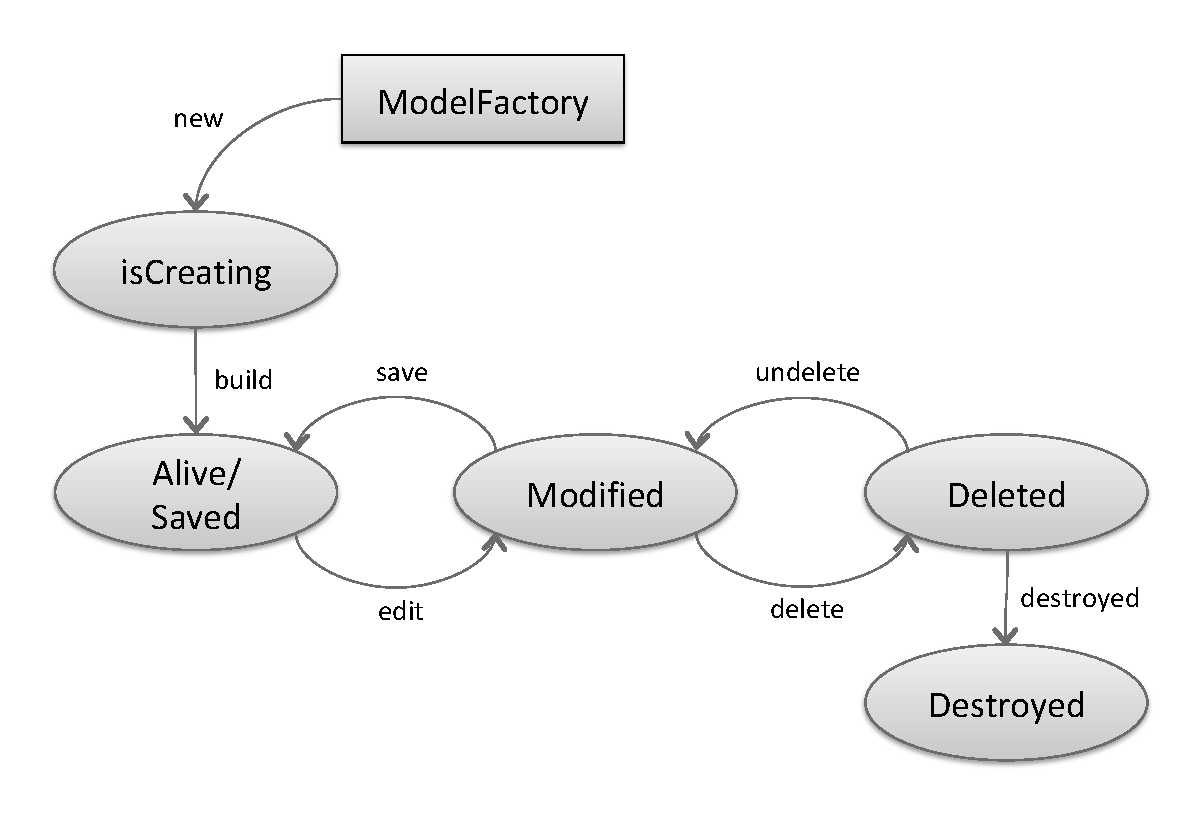
\includegraphics[width=0.9 \columnwidth]{LifeCycle.pdf}
    \caption{Life-cycle of PAMELA objects}
    \label{fig:LifeCycle}
\end{figure}

Modifications of objects are internally tracked by PAMELA interpreter which manages \mytexttt{Modified} status, according to containment semantics as presented further (a contained object modification implies object flagged as modified, and implied container flaggued as modified too). Saving object graph brings back object status in \mytexttt{Alive/Saved} status.

Since calls to any features of model objects are dispatched by the internal interpreter, PAMELA runtime offers a multi-level undo/redo stack tooling. When enabled, this scheme allows to store and manage an edition model composed of atomic edits. Figure \ref{fig:AtomicEditMetaModel} presents atomic edits metamodel for a fine-grained model modification tracking system. That mechanism provides undo/redo features, virtually unlimited. For performance reasons, we can set a maximum depth for undo/redo operations.

\begin{figure}
    \centering
    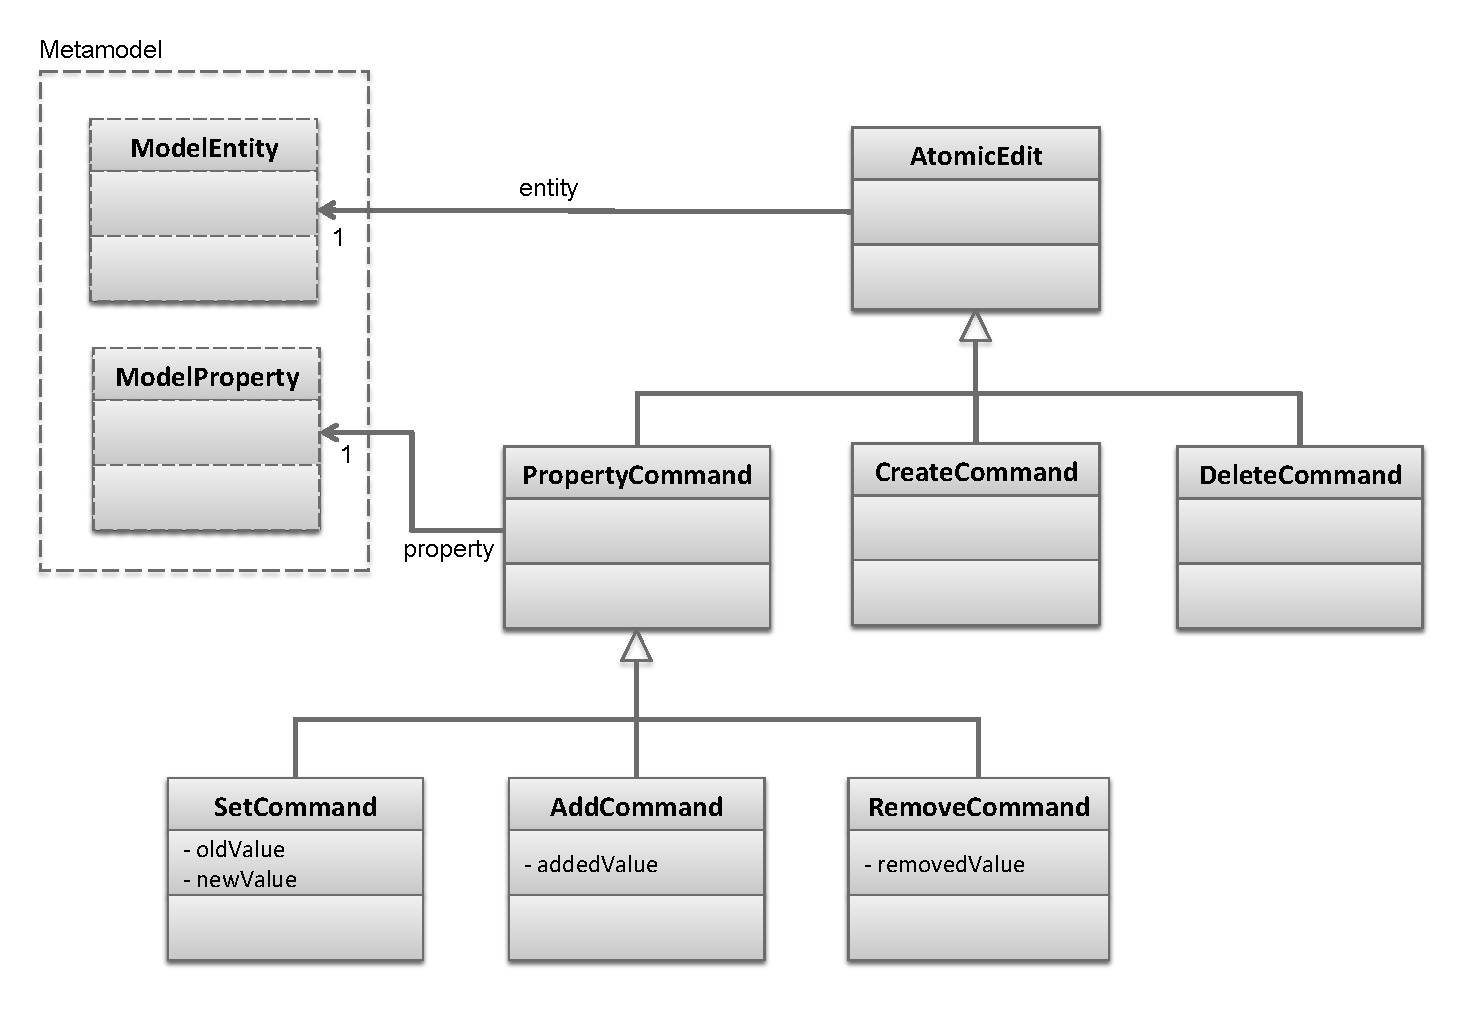
\includegraphics[width=1.0 \columnwidth]{AtomicEditMetaModel.pdf}
    \caption{Atomic edits metamodel}
    \label{fig:AtomicEditMetaModel}
\end{figure}

\mytexttt{DeletableProxyObject} provides delete (and undelete) features to \emph{ModelEntity} instances. Deletion features are performed using a context which is a graph closure computation for all the objects which have to be deleted. PAMELA also offers undelete feature which allow to resurrect a deleted object. Deleted objects are still resurectable until they are still in the undo/redo stack. A deleted object who is leaving scope of maximum depth of undo/redo stack is destroyed. Object is fully dereferenced, ready for garbage collecting, and cannot be resurrected again.

\subsection{Meta-programming support}

Figure \ref{fig:PamelaMetaModel} represents PAMELA metamodel. Concept of \emph{ModelProperty} represent access to a value (simple or with multiple cardinality). This read-access is implicitely implemented using \mytexttt{get:} protocol. Following the same logic, PAMELA properties may expose following protocols:
\begin{itemize}
    \item \mytexttt{get:} read-access to a data. This protocol is implemented by all kind of \emph{ModelProperties}.
    \item \mytexttt{set:} write-access to a data. This protocol is implemented by \emph{ModelProperties} implementing \mytexttt{SettablePropertyImplementation} API.
    \item \mytexttt{add:} and \mytexttt{add:AtIndex:} add-access to a multiple cardinality data. These protocols are implemented by \emph{ModelProperties} implementing \mytexttt{MultiplePropertyImplementation} API.
    \item \mytexttt{remove:} remove-access to a multiple cardinality data. This protocols is implemented by \emph{ModelProperties} implementing \mytexttt{MultiplePropertyImplementation} API.
    \item \mytexttt{delete:} and \mytexttt{undelete:} delete/undelete protocols, implemented by all \emph{ModelProperties}
\end{itemize}

Unless specified in \mytexttt{@PropertyImplementation} PAMELA annotations, default implementation are provided the PAMELA interpreter. Default implementations are encoded in well identified classes which are extendable. 

PAMELA allows programmers to define their custom implementation for a given set of properties, while providing a class implementing \mytexttt{@PropertyImplementation} API and some protocol implementation (depending on the nature of the \emph{ModelProperty}. Following excerpt of code illustrate use of two custom property implementations.

\begin{lstlisting}[language=Java,basicstyle=\ttfamily\footnotesize]
@ModelEntity
public interface MyConcept {

	static final String VALUE = "value";
	static final String SUB_CONCEPTS = "someSubConcepts";

	@Getter(value = VALUE)
	@PropertyImplementation(MyPropertyImplementation.class)
	String getValue();

	@Setter(VALUE)
	public void setValue(String value);

	@Getter(value = SUB_CONCEPTS, cardinality = Cardinality.LIST)
	@PropertyImplementation(MyListCardinalityPropertyImplementation.class)
	@Embedded
	List<MySubConcept> getSubConcepts();

	@Adder(SUB_CONCEPTS)
	void addToSubConcepts(MySubConcept subConcept);

	@Remover(SUB_CONCEPTS)
	void removeFromSubConcepts(MySubConcept subConcept);
}

public class MyPropertyImplementation extends DefaultSinglePropertyImplementation<Concept, String> {

	public MyPropertyImplementation(ProxyMethodHandler<Concept> handler, ModelProperty<Concept> property)
			throws InvalidDataException {
		super(handler, property);
	}

    // Implements get: protocol
    // ('concatenate' semantics)
	@Override
	public void set(String aValue) throws ModelDefinitionException {
		String oldValue = get();
		if (get() != null) {
			super.set(aValue + get());
		}
		else {
			super.set(aValue);
		}
	}
}

public class MyListCardinalityPropertyImplementation<I, T> extends AbstractPropertyImplementation<I, List<T>>
		implements MultiplePropertyImplementation<I, T> {
	...
	// Implements get: protocol
	public List<T> get() {
		...
	}
	// Implements add: protocol
	public void addTo(T aValue) throws ModelDefinitionException {
		...
	}
	// Implements remove: protocol
	public void removeFrom(T aValue) {
		...
	}
}
\end{lstlisting}

Such mechanisms are really usefull to control and fine-tune code implementation. Suppose for example that you have a code used in monothreading context: all your multiple cardinality properties will rely for example on a \mytexttt{ArrayList} implementation. Instead of replacing all occurences of \mytexttt{ArrayList} by \mytexttt{Vector} (multi-thread safe version of Java \mytexttt{List}) in generated code, the developer has just one modication to do, in adequate \mytexttt{PropertyImplementation}.

\subsection{Multiple inheritance and traits programming}

\begin{lstlisting}[language=Java,basicstyle=\ttfamily\footnotesize]
@ModelEntity
public interface IntegerStorage extends AccessibleProxyObject {

     public static final String STORED_VALUE = "storedValue";

     @Getter(value = STORED_VALUE, defaultValue = "-1")
     public int getStoredValue();

     @Setter(value = STORED_VALUE)
     public void setStoredValue(int aValue);

     public void reset();

     @Implementation
     public abstract class IntegerStorageImpl implements IntegerStorage {
	@Override
	public void reset() {
	     setStoredValue(0);
	}

	@Override
	public void setStoredValue(int aValue) {
	     performSuperSetter(STORED_VALUE, aValue);
	     System.out.println("Sets stored value to be " + aValue);
	}
    }
}

@ModelEntity
public interface PlusProcessor extends IntegerStorage {

     public void processPlus(int value);

     @Implementation
     public abstract class PlusProcessorImpl implements PlusProcessor {
	@Override
	public void processPlus (int value) {
	     setStoredValue(getStoredValue()+value);
	     return getStoredValue();
	}
     }
}

@ModelEntity
public interface MinusProcessor extends IntegerStorage {

     public void processMinus(int value);

     @Implementation
     public abstract class MinusProcessorImpl implements MinusProcessor {
	@Override
	public void processMinus (int value) {
	     setStoredValue(getStoredValue()-value);
	     return getStoredValue();
	}
     }
}

@ModelEntity
public interface Calculator extends PlusProcessor, MinusProcessor {

}

\end{lstlisting}

\subsection{Embedding management and cloning support}

- embedding support
- cloning support (closure computation)
- clipboard operations

\subsection{Notification support}

- notification support
- isModified() support (embedding semantics)

\subsection{Persistance support}

- XML serialization/deserialization

\subsection{Graph computation features}

- support for computing equality
- diff/merge support, updateWith()
- visiting support



\subsection{Support for Contrat Programming}

- design by contract
- contract programming (JML)

% reference to jContractor

\subsection{Design patterns / Aspect programming / Code weaving}

- design patterns / aspect programming / code weaving



